%=============================================================================
%  CS3631 Phase 3 -- Full Paper
%  PAGE: persistence-anchored gated forecasting for district-level dengue
%  Group 05, Department of Computer Science and Engineering, University of Moratuwa
%
%  Rewritten 2026-09-24 on the corrected dataset and the leakage-controlled
%  harness (seirgnn2/). Restructured 2026-10-07 to the CS3631 brief (section 9)
%  and the lecturer's paper-writing feedback: a named framework (PAGE), its
%  formal description, ablation, comparative analysis, tuning, computational
%  analysis and the prospective 2024-2026 test (EXP-063).
%  Every number in tables_generated.tex and the fig_* files comes from
%  scripts/build_paper_assets.py (Kaggle run, EXP-050); tables_extra.tex comes
%  from scripts/build_paper_extra_tables.py (EXP-063 and the same Kaggle run).
%  Numbers in the prose must match them.
%
%  CONTRIBUTION COLOURS: the rewrite was done in one pass, so the \cA..\cF
%  wrappers are not applied to the new text. Re-assign them at the team standup
%  before building main-highlighted.pdf.
%
%  BUILD:
%    make              -> main.pdf            (clean version, for submission)
%    make highlighted  -> main-highlighted.pdf (colour-coded contributions, for grading)
%
%  Both versions come from THIS FILE. Never fork the text.
%=============================================================================
\documentclass[sigconf,nonacm]{acmart}

%--- Contribution highlighting -----------------------------------------------
% Toggled by the build. Do not edit by hand; `make highlighted` sets it.
\newif\ifhighlight
\ifdefined\HIGHLIGHTON\highlighttrue\else\highlightfalse\fi

\usepackage{xcolor}
\usepackage{soul}
% todonotes needs margin room; acmart gives it almost none by default.
\setlength{\marginparwidth}{2cm}
\usepackage[textsize=tiny]{todonotes}

% One colour per member.
\definecolor{colTharusha}{RGB}{255,236,153}   % yellow
\definecolor{colPraveenD}{RGB}{183,225,205}   % green
\definecolor{colJanith}  {RGB}{255,204,204}   % pink
\definecolor{colBimsara} {RGB}{204,224,255}   % blue
\definecolor{colMaleesha}{RGB}{229,204,255}   % purple
\definecolor{colPraveenN}{RGB}{255,224,178}   % orange

% \cA{...} .. \cF{...} wrap text belonging to a member.
% In the clean build they are invisible no-ops.
\ifhighlight
  \newcommand{\cA}[1]{{\sethlcolor{colTharusha}\hl{#1}}}
  \newcommand{\cB}[1]{{\sethlcolor{colPraveenD}\hl{#1}}}
  \newcommand{\cC}[1]{{\sethlcolor{colJanith}\hl{#1}}}
  \newcommand{\cD}[1]{{\sethlcolor{colBimsara}\hl{#1}}}
  \newcommand{\cE}[1]{{\sethlcolor{colMaleesha}\hl{#1}}}
  \newcommand{\cF}[1]{{\sethlcolor{colPraveenN}\hl{#1}}}
  % Margin note for "X implemented it, Y wrote it up" cases. REQUIRED by the brief.
  \newcommand{\credit}[1]{\todo[size=\tiny,color=gray!20]{#1}}
\else
  \newcommand{\cA}[1]{#1}\newcommand{\cB}[1]{#1}\newcommand{\cC}[1]{#1}
  \newcommand{\cD}[1]{#1}\newcommand{\cE}[1]{#1}\newcommand{\cF}[1]{#1}
  \newcommand{\credit}[1]{}
\fi

%--- Packages ----------------------------------------------------------------
\usepackage{booktabs}
\usepackage{amsmath}
\let\Bbbk\undefined
\usepackage{amssymb}
\usepackage{graphicx}
\usepackage{subcaption}
\usepackage{balance}
\usepackage{tikz}
\usetikzlibrary{positioning,arrows.meta,fit,calc}

% Notation shorthands -- keep the maths consistent across sections.
\newcommand{\R}{\mathbb{R}}
\newcommand{\Rhat}{\hat{R}}
\newcommand{\padj}{p_{\text{adj}}}
% The framework's name. Change it here and everywhere follows.
\newcommand{\model}{PAGE}
% Anonymised code link for double-blind venues (anonymous.4open.science mirrors
% the GitHub repository). TODO: create the mirror and replace before submission.
\newcommand{\codeurl}{\url{https://anonymous.4open.science/r/TODO}}

% NOTE: do NOT add authorsperrow here. With six authors sharing ONE \affiliation,
% acmart keeps them in a single box, so authorsperrow only narrows that box --- it
% squeezes the affiliation and pushes the shared email line past the right margin.
\settopmatter{printacmref=false}
\setcopyright{none}
\renewcommand\footnotetextcopyrightpermission[1]{}
\pagestyle{plain}

%=============================================================================
\begin{document}

% TITLE. Names the framework and its key idea (the lecturer's rule). The
% question mark keeps the claim honest: on unseen weeks nothing beats
% persistence on RMSE (Table tab:prospective).
\title{Beyond Persistence? \model{}: Persistence-Anchored Gated Forecasting\\
with Spatio-Temporal Graph Networks for Dengue}

% AUTHORS. Phase 3 requires TAs then Prof.\ Dulani and Dr.\ Sandareka appended
% as final co-authors -- add them before submission.
\author{Tharusha Perera}
\author{Praveen De Silva}
\author{Janith Mahanama}
\author{Bimsara Udurawana}
\author{Maleesha Kumarasinghe}
\author{Praveen Nawarathna}
\affiliation{%
  \institution{Department of Computer Science and Engineering, University of Moratuwa}
  \city{Moratuwa}
  \country{Sri Lanka}
}
\email{{tharushap.23,praveend.23,janithm.23,bimsarau.23,kumarasinghemp.23,praveenn.23}@cse.mrt.ac.lk}

%=============================================================================
% ABSTRACT
% Flow (lecturer's feedback): background -> technical gap in existing work ->
% proposed framework -> key results -> code link.
%=============================================================================
\begin{abstract}
Dengue causes recurring epidemics in Sri Lanka, and district-level forecasts three
weeks ahead give health services time to act. Spatio-temporal graph neural networks
(ST-GNNs) and SEIR-informed neural models have been proposed for this task, but both
predict the case level directly and are evaluated without the naive persistence
forecast, on a benchmark array that we show leaks future data. On this target last
week's count explains $r^2=0.89$ of the next and the best climate covariate $0.03$,
so a direct head must relearn an identity map through its encoder, and several
published ST-GNNs fail to. We propose \model{} (Persistence-Anchored Gated
Estimation), a forecasting head that plugs into any spatio-temporal encoder and
predicts a gated departure from the last observed week, at the cost of one
parameter. We rebuild a leakage-free 559-week dataset from hash-verified sources,
extend it to August 2026, and evaluate five published ST-GNNs and the LSTM of
SEIR-LSTM on one pre-registered harness. \model{} repairs the three encoders that
fail as published by 5.95--16.29 validation RMSE and 23.24--34.50 test RMSE (9/9
paired runs each), and on AAGCN it beats persistence on all 9 runs on both splits. An
ablation attributes the gain to the anchor and the gate: an SEIR simulator in the
same head adds nothing, and on 85 unseen forecast starts it ties its no-SEIR twin
($\Delta=-0.03$, $p=0.67$). On those unseen weeks no learned model beats persistence
on RMSE (34.75 against 35.43 for \model{}), although \model{} has lower MAE and
SMAPE. On this target the useful prior is persistence, not transmission dynamics.
Code and data: \codeurl.
\end{abstract}


\keywords{dengue forecasting, spatio-temporal graph neural networks,
persistence, SEIR, physics-informed learning, data leakage, prospective
evaluation, negative results}

\maketitle

%=============================================================================
% INTRODUCTION
% Flow (CS3631 brief, section 9): background -> technical issue not addressed
% by existing work -> proposed solution, briefly -> main results -> 3 contributions.
%=============================================================================
\section{Introduction}
\label{sec:intro}

Dengue is the fastest-spreading mosquito-borne viral disease, and Sri Lanka
faces recurring severe epidemics: the 2017 outbreak alone recorded over 186{,}000
cases and 440 deaths~\cite{tissera2020severe}. Roughly three weeks separate
infection from diagnosis, so district-level forecasts issued $H=3$ weeks ahead
give clinicians and vector-control teams time to prepare beds and target spraying.

Two families of deep model are proposed for this task. Spatio-temporal graph
neural networks (ST-GNNs), transferred from traffic forecasting, treat districts
as nodes and learn from neighbours; Weng et al.~\cite{weng2024graph} benchmark five
of them on Sri Lanka's weekly record. SEIR-informed models push the forecast through
compartmental dynamics; Liu et al.~\cite{liu2025seirlstm} drive an SEIR model with an
LSTM on the same country. The natural hybrid, an SEIR-GNN, replaces that LSTM with a
graph encoder.

\textbf{The technical gap.} Weekly dengue incidence is close to a random walk. On the
corrected data, cases at $t-1$ explain $r^2=0.89$ of cases at $t$; the best single
climate covariate at a causal lag explains $0.03$. Both model families nevertheless
predict the case \emph{level} directly from an encoder representation, so the network
must relearn the identity map $\hat y_{t+1}\approx y_t$ through its message passing
and recurrence before it can add anything. We find that three of the five published
ST-GNNs do not: they underfit, and on validation are 5--17 RMSE worse than simply
repeating last week. The benchmark that reports them hides this, because it omits the persistence
forecast $\hat y_{t+h}=y_t$ and its array leaks future data
(\S\ref{sec:audit}). Neither line of work tests its physics or its graph against a
matched control that differs in that component alone.

\textbf{Proposed solution.} We propose \model{} (Persistence-Anchored Gated
Estimation), a forecasting head that plugs into any spatio-temporal encoder. It
starts from the persistence forecast and lets the network supply only a
\emph{departure} from it, scaled by a learned gate initialised near zero. The
identity map is therefore free, the network learns only what persistence misses,
and the gate shrinks that correction until the data support it. \model{} adds one
parameter. Its departure can come from a linear read-out or from a differentiable
SEIR simulator, which lets one controlled ablation ask whether physics helps.

\textbf{Main results.} On one leakage-free harness (Figure~\ref{fig:overview},
Table~\ref{tab:encoders}), \model{} repairs STGAT, A3TGCN and DCRNN by 5.95--16.29
validation RMSE (9/9 paired runs each), and with AAGCN it beats persistence on all
9 runs on validation and on test. The ablation (Table~\ref{tab:rescue}) attributes the
gain to the anchor and the gate; an SEIR departure adds nothing. On 85 forecast starts
from March 2024 to August 2026, scored with settings frozen before those weeks were
parsed, the SEIR branch ties \model{} ($p=0.67$) and no learned model beats persistence on
RMSE, although \model{} has lower MAE and SMAPE (Table~\ref{tab:prospective}). We report
this negative result as it is.

\noindent\textbf{Contributions.}
\begin{enumerate}\itemsep1pt
  \item \textbf{\model{}, a persistence-anchored gated head} (\S\ref{sec:framework}),
        encoder-agnostic and one parameter in size, that makes every published
        ST-GNN we test usable and isolates, by ablation, where the gain comes from:
        the anchor and the gate, not the physics.
  \item \textbf{A leakage-free dataset} (\S\ref{sec:data}). We audit the benchmark
        array, which mixes time orders, trains on post-test data and feeds future
        rainfall as a ``lagged'' feature, and correct it into a 559-week (2013--2024)
        leakage-free series, extended with 127 newly parsed 2024--2026 reports for
        a prospective test.
  \item \textbf{A controlled and prospective evaluation} (\S\ref{sec:experiments}):
        six encoders, matched no-physics and no-graph controls, paired tests,
        pre-registered decision rules and a prospective 2024--2026 test. It shows that
        the graph adds 0.06 RMSE, the SEIR branch adds nothing, and the remaining
        error is informational rather than architectural.
\end{enumerate}

%=============================================================================
% RELATED WORK
%=============================================================================
\section{Related Work}
\label{sec:related}

\textbf{ST-GNNs for epidemics and dengue.} Spatio-temporal graph networks couple a
graph operator over regions with a temporal operator over history. The five we
evaluate come from traffic forecasting. STGAT and A3TGCN~\cite{bai2021a3tgcn}
use attention, ASTGCN~\cite{guo2019astgcn} attends over space and time,
AAGCN~\cite{shi2019aagcn} adapts its adjacency, and DCRNN~\cite{li2018dcrnn}
diffuses over the graph inside a recurrent cell; Graph WaveNet~\cite{wu2019graphwavenet}
learns the adjacency from node embeddings. For epidemics, Cola-GNN~\cite{deng2020colagnn}
and EpiGNN~\cite{xie2022epignn} add cross-location attention and transmission-risk
encodings. Weng et al.~\cite{weng2024graph} benchmark the five traffic ST-GNNs on Sri
Lanka's dengue record, and GulMohamed et al.~\cite{gulmohamed2026denguegnn} add
per-horizon heads, temporal attention and a Gaussian output. All of them predict the
case level directly, and the dengue benchmark~\cite{weng2024graph} reports no
persistence baseline.

\textbf{Mechanistic hybrids.} Liu et al.~\cite{liu2025seirlstm} forecast Sri Lankan
dengue with an SEIR model whose force of infection is predicted by an LSTM; we call
this SEIR-LSTM. EINNs~\cite{rodriguez2023einns} couple a neural forecaster with a
mechanistic model through shared latent dynamics. CausalGNN~\cite{wang2022causalgnn}
and MepoGNN~\cite{cao2023mepognn} embed a metapopulation SEIR in a graph network, so
that districts are coupled inside the dynamics. Physics-informed
networks~\cite{raissi2019pinn} add dynamics as a loss; MP-PINN~\cite{nguyen2024mppinn}
applies this to epidemic curves. We use the SEIR--SEI stage durations of Phaijoo and
Gurung~\cite{phaijoo2018sensitivity}. These works compare against purely data-driven
models, but not against the same head with the simulator removed, so the share of
the gain that is due to physics is not measured.

\textbf{Persistence and simple baselines.} In classical forecasting the naive forecast
$\hat y_{t+h}=y_t$ is the reference every method must beat, and differencing, which
models the change rather than the level, is the standard treatment of a series close
to a random walk~\cite{hyndman2021forecasting}. In deep
spatio-temporal forecasting, simple models often match complex ones:
STID~\cite{shao2022stid} replaces graph operators with identity embeddings.
Reversible instance normalisation~\cite{kim2022revin} targets distribution shift,
count likelihoods such as the negative binomial of DeepAR~\cite{salinas2020deepar}
target skewed counts, and TimeGAN~\cite{yoon2019timegan} generates synthetic
sequences. \model{} brings the classical idea into the ST-GNN head: it anchors on
persistence and learns a gated departure. We also test each of the remedies above
under the same protocol.

%=============================================================================
% DATASET CONSTRUCTION (a contribution, so it is described as methodology,
% per the lecturer's feedback; Section 5.1 gives only the overview)
%=============================================================================
\section{Dataset Construction}
\label{sec:data}

\subsection{Reproducing the benchmark}
\label{sec:repro}
We first ran the reference implementation~\cite{weng2024graph} unmodified (their
code, array and protocol) on a pinned software stack. It recovers their published
numbers to within \textbf{7.3\%} across twenty comparisons. Three properties of their
evaluation, however, account for the reported advantage: the ``cross validated''
column is computed on a loader that includes training data; RMSE is averaged per
window rather than pooled, which on this target is $\sim$39\% lower; and no naive
baseline is reported. Adding persistence to that same column reverses the ranking:
it beats \emph{every} model on MAE and RMSE. An independent re-implementation that
shares no code with either codebase reproduces this.

\subsection{Auditing the benchmark array}
\label{sec:audit}
The benchmark array (\texttt{sri\_lanka\_2013-2022\_shifted.npy}) has no date
axis. We dated every row by matching its 25 district counts exactly against the
weekly reports, and dated the weather channels separately by finding the
calendar offset at which the array's temperature best matches ERA5.
Table~\ref{tab:audit} lists what that shows.

\begin{table}[t]
\centering
\caption{Audit of the benchmark array, recomputed by the reproduction notebook
from the original files.}
\label{tab:audit}
\small
\setlength{\tabcolsep}{3pt}
\begin{tabular}{p{0.33\linewidth}p{0.57\linewidth}}
\toprule
finding & consequence \\
\midrule
Rows 0--47 are Dec 2022--Nov 2023; rows 51 onward run 2013--2022 & 45 rows from 2023 sit in
the training split of every fold, which tests on 2018--2022 \\
Cases reordered, weather not & the array's temperature matches ERA5 at
$r = 0.95$ on its own row order and $r = 0.45$ on the dates the case rows carry \\
``Lag 12'' precipitation & matches ERA5 rain 12 weeks \emph{later}
($r = 0.68$) and not 12 weeks earlier ($r = 0.19$): future information \\
48 reports dropped, one week stored twice & 454 of 459 rows equal a published
report exactly \\
Week-395 spike & row A of one printed table is a dragged formula
(15 of 24 cells are the sum of the two before, districts sum to 7,165 against a
national cell of 35); the same table's cumulative row gives the true count \\
\bottomrule
\end{tabular}
\end{table}

Two of these are information leaks. Training on 2023 while testing on
2018--2022 lets a model see the future of its test period, and a ``lagged''
rainfall channel that holds rain from twelve weeks ahead gives it that future's
weather. Any score on this array, including the published ones and our own
earlier work, is therefore an optimistic bound. Earlier drafts of this study
called the week-395 spike an administrative reporting backlog. It is a
spreadsheet error, and it can be corrected from the same published table.

\subsection{The corrected dataset}
\label{sec:corrected}
The 2013--2024 case counts come from the benchmark authors' table of parsed
Table~1 rows of every Weekly Epidemiological Report; we do not re-parse those
reports. The other inputs we obtain ourselves: the one report PDF used for the
correction, ERA5 daily responses from the Open-Meteo archive, and the Department
of Census and Statistics population and census PDFs. Every input file has a
recorded SHA-256 checksum. From these the case series is re-dated, keyed by report volume
and number: 559 weeks from 2013-W26 to 2024-W10. The seven weeks with no report
stay missing and are never interpolated; districts plus the Kalmunai division
equal the Epidemiology Unit's own national total in 432 of 552 reports. Weekly
ERA5 temperature, precipitation, humidity and soil moisture are aggregated from
daily values at an interior point of each district, and each week's population
is the latest official figure for an earlier year (the 2012 Census, whose 25
district totals sum exactly to the national total, then mid-year estimates).

Lags are applied in the model, not baked into the data: a forecast for week $t$
reads cases up to $t-1$ and climate up to $t-2$, since ERA5 is published about
five days late. The lags are enforced in code, and for the data loader used in the
prospective test a perturbation test asserts that no value after either limit can
change a forecast. On this series the persistence test RMSE on the three
development origins (\S\ref{sec:protocol}) is \textbf{36.02}, against 44.80 on the
array (29.52 with the week-395 windows excluded). The last test fold covers the
2023 epidemic.

\subsection{Extension to 2026 for a prospective test}
\label{sec:newweeks}
To test on weeks that no design decision had seen, we extend the series with the 127
Weekly Epidemiological Reports from 2024-W11 to 2026-W32. The parsing and quality
rules (district totals must match the national total; a dragged-formula pattern
or a reprinted table voids a week's row, which is then replaced by the difference of
the cumulative rows or left missing) were committed before any count was read. The
result is 109 observed weeks, 8 corrected and 10 missing; nothing is interpolated.
One deviation is reported in full: a first scoring run exposed two reconstruction
defects (the first report of a year carries the previous year's total in its
cumulative row, and two reports reprint the previous week's table). The rules were
amended on report semantics alone, no model setting changed, and only the
re-parsed data are scored (\S\ref{sec:prospective}). This is therefore an amended
prospective evaluation, not an untouched one.

%=============================================================================
% THE PAGE FRAMEWORK
% Lecturer's feedback: symbols only (numbers go in Implementation Details),
% start from the input, show every step to the output, then the loss.
%=============================================================================
\section{The \model{} Framework}
\label{sec:framework}

\begin{figure*}[t]
\centering
\begin{tikzpicture}[
  font=\small, >={Stealth[length=2mm]},
  box/.style={draw, rounded corners=2pt, align=center, minimum height=9mm, inner sep=3pt, fill=white},
  inp/.style={box, fill=gray!8},
  key/.style={box, fill=teal!12, draw=teal!70!black, line width=0.8pt},
  opt/.style={box, dashed, fill=orange!8},
  op/.style={circle, draw, inner sep=1pt, minimum size=5mm},
  lbl/.style={font=\scriptsize, inner sep=1pt}]
  % inputs (left)
  \node[inp] (x) {case window\\$\mathbf{Z}_t\in\R^{N\times W}$};
  \node[inp, above=3mm of x] (a) {district graph\\$\mathcal{G}=(\mathcal{V},\mathcal{E},\mathbf{A})$};
  \node[inp, above=3mm of a] (e) {covariates (opt.)\\$\mathbf{E}_t\in\R^{N\times F}$};
  % encoder
  \node[box, right=9mm of x, minimum width=24mm] (enc) {encoder $f_\theta$\\{\scriptsize any ST-GNN or LSTM}};
  \node[box, right=7mm of enc] (ro) {read-out\\$\mathbf{u}_i=\mathbf{W}\tilde{\mathbf{h}}_i+\mathbf{b}$};
  \node[opt, above=4mm of ro] (seir) {SEIR branch (ablated)\\$\mathbf{u}_i=\mathrm{SEIR}(\lambda_i;\,\mathbf{s}_{i,t})$};
  % PAGE head
  \node[op, right=10mm of ro] (minus) {$-$};
  \node[key, right=6mm of minus] (gate) {gate\\$g=\sigma(a)$};
  \node[op, right=6mm of gate] (plus) {$+$};
  \node[box, right=7mm of plus] (out) {forecast\\$\hat{\mathbf{y}}_i\in\R^{H}$};
  % anchor path
  \node[key, below=9mm of minus] (anc) {persistence anchor $p_i=z_{i,t}$};
  % arrows
  \draw[->] (x) -- (enc);
  \draw[->] (a.east) -| ($(enc.north west)!0.3!(enc.north east)$);
  \draw[->] (e.east) -| ($(enc.north west)!0.7!(enc.north east)$);
  \draw[->] (enc) -- node[lbl, below, pos=0.3]{$\tilde{\mathbf{h}}_i$} (ro);
  \coordinate (br) at ($(enc.east)!0.6!(ro.west)$);
  \draw[->, dashed] (br) -- (br |- seir.south);
  \draw[->] (ro) -- node[lbl, above]{$\mathbf{u}_i$} (minus);
  \draw[->, dashed] (seir.east) -| (minus.north);
  \draw[->] (minus) -- node[lbl, above]{$\boldsymbol{\delta}_i$} (gate);
  \draw[->] (gate) -- (plus);
  \draw[->] (plus) -- node[lbl, above]{$\hat{\mathbf{z}}_i$} (out);
  \draw[->] (x.south) |- (anc.west);
  \draw[->] (anc) -- (minus);
  \draw[->] (anc.east) -| (plus.south);
  % highlight the contribution
  \node[draw=teal!70!black, dotted, rounded corners, inner sep=2.5mm, fit=(minus)(gate)(plus)(anc),
        label={[font=\scriptsize\bfseries, text=teal!50!black]above:\model{} head (our contribution)}] {};
\end{tikzpicture}
\caption{\model{}. An unchanged encoder reads the last $W$ weeks of standardised log cases
on the district graph. Its read-out $\mathbf{u}_i$ is turned into a departure
$\boldsymbol{\delta}_i=\mathbf{u}_i-p_i\mathbf{1}$ from the persistence anchor, shrunk by
a learned gate, and added back to the anchor. The dashed SEIR branch replaces the
read-out with a differentiable simulator; it is the component the ablation removes.}
\label{fig:overview}
\end{figure*}

\subsection{Problem formulation}
Let $\mathcal{G}=(\mathcal{V},\mathcal{E},\mathbf{A})$ be the district graph with
$|\mathcal{V}|=N$ districts and adjacency $\mathbf{A}\in\{0,1\}^{N\times N}$ (with
self-loops), and let $y_{i,t}\ge 0$ be the dengue cases reported by district $i$ in
week $t$. Counts are modelled on the scale
$z_{i,t}=(\log(1+y_{i,t})-m)/s$, where $m$ and $s$ are the mean and standard deviation
of $\log(1+y)$ over the training weeks only. At forecast origin $t$ the input is the
window $\mathbf{Z}_t=[z_{i,t-W+1},\dots,z_{i,t}]_{i\in\mathcal{V}}\in\R^{N\times W}$ and,
optionally, exogenous covariates $\mathbf{E}_t\in\R^{N\times F}$ observed at causal
lags (\S\ref{sec:corrected}). The task is to predict
$\mathbf{Y}_t=[y_{i,t+h}]\in\R^{N\times H}$ for horizons $h=1,\dots,H$.

\subsection{Encoder}
Any spatio-temporal encoder $f_\theta$ maps the window to one representation per
district,
\begin{equation}
  \mathbf{H}=f_\theta(\mathbf{Z}_t,\mathbf{A})\in\R^{N\times d},\qquad
  \tilde{\mathbf{h}}_i=[\mathbf{h}_i\,\Vert\,\mathbf{e}_{i,t}],
\end{equation}
where $\Vert$ concatenates any covariates around the encoder, so that a published
architecture runs exactly as designed. We use the five published ST-GNNs and the LSTM
of SEIR-LSTM unchanged (\S\ref{sec:baselines}). A linear read-out gives a level
forecast $\mathbf{u}_i=\mathbf{W}\tilde{\mathbf{h}}_i+\mathbf{b}\in\R^{H}$; the
published models stop here and output $\hat{\mathbf{z}}_i=\mathbf{u}_i$ (the
\emph{direct} head).

\subsection{Persistence-anchored gated head}
\label{sec:page}
\model{} anchors every horizon on the last observed week, $p_i=z_{i,t}$, and lets the
network contribute only a gated departure from it:
\begin{equation}
  \boldsymbol{\delta}_i=\mathbf{u}_i-p_i\mathbf{1}_H,\qquad
  \hat{\mathbf{z}}_i=p_i\mathbf{1}_H+g\,\boldsymbol{\delta}_i,\qquad g=\sigma(a),
  \label{eq:page}
\end{equation}
with one learned scalar $a$, initialised at $a_0<0$ so that training starts close to
the persistence forecast. Equivalently
$\hat{\mathbf{z}}_i=(1-g)\,p_i\mathbf{1}_H+g\,\mathbf{u}_i$: a learned convex
combination of persistence and the encoder's forecast. Counts are recovered as
$\hat y_{i,t+h}=\max\!\big(0,\exp(s\,\hat z_{i,h}+m)-1\big)$.

\textbf{Design rationale.} Three properties follow from Eq.~\eqref{eq:page}.
(i)~\emph{The identity is free.} At $g\to0$ the model is exactly persistence, which
already explains $r^2=0.89$ of the next week; a direct head must instead carry the
level through the encoder's message passing and recurrence, and the three failing
encoders do not (\S\ref{sec:comparative}). (ii)~\emph{The gate is a learned
shrinkage.} The gradient raises $g$ only as far as $\mathbf{u}_i$ improves on $p_i$,
so a weak encoder cannot pull the forecast far from a strong baseline. (iii)~\emph{It
costs one parameter} and no extra computation (Table~\ref{tab:compute}). Removing the
gate ($g\equiv1$, $\hat{\mathbf{z}}_i=p_i\mathbf{1}_H+\boldsymbol{\delta}'_i$ with an
unconstrained departure) gives the \emph{residual} head, and removing the anchor gives
the direct head; both are ablations in \S\ref{sec:ablation}.

\subsection{Optional SEIR branch}
\label{sec:seirbranch}
To test whether transmission dynamics help, the read-out can be replaced by a
differentiable SEIR model. The encoder predicts a weekly force of infection
$\lambda_{i,h}=\min\!\big(\exp(\mathbf{w}^{\top}\tilde{\mathbf{h}}_i+b_\lambda),\,
\lambda_{\max}\big)$, and the compartments
$\dot S=-\lambda S$, $\dot E=\lambda S-\omega E$, $\dot I=\omega E-\gamma I$,
$\dot R=\gamma I$ are stepped daily from a state $\mathbf{s}_{i,t}$ seeded by observed
cases (exposed and infectious from the counts of weeks $t-1$ and $t$, divided by a
reporting rate $\rho$; susceptibles from a serosurvey). Weekly incidence $\iota_{i,h}$ (the flow $E\to I$) times $\rho$ times the
district population $P_i$ gives counts, so
$u_{i,h}=(\log(1+\rho P_i\iota_{i,h})-m)/s$, which enters Eq.~\eqref{eq:page} in place
of the read-out; learned scales on the seeded exposed state and on $\rho$ are allowed.
With the anchor and gate this is the SEIR-GNN (or SEIR-LSTM when $f_\theta$ is the
LSTM); without them, $\hat{\mathbf{z}}_i=\mathbf{u}_i$, it is a pure SEIR decoder.

\subsection{Learning objective}
\label{sec:loss}
All parameters $\Theta=\{\theta,\mathbf{W},\mathbf{b},a\}$ (plus $\mathbf{w},b_\lambda$
and the SEIR scales when the branch is used) minimise the squared error on the
standardised scale over a mini-batch $\mathcal{B}$ of forecast origins,
\begin{equation}
  \mathcal{L}(\Theta)=\frac{1}{|\mathcal{B}|\,N H}\sum_{t\in\mathcal{B}}\sum_{i=1}^{N}
  \sum_{h=1}^{H}\big(\hat z_{i,h}^{(t)}-z_{i,t+h}\big)^2 ,
\end{equation}
with early stopping on validation RMSE in counts. We also test a negative-binomial
(NB) objective, which adds a dispersion head and minimises the NB2 negative
log-likelihood with mean $\mu=\exp(s\hat z+m)-1$. The reason is a bias: under squared
error on $\log(1+y)$, $\exp$ of the fit is a conditional \emph{median}, while RMSE
rewards the conditional \emph{mean}, which NB's $\mu$ estimates.

\subsection{Implementation details}
\label{sec:impl}
$N=25$ districts, window $W=3$, horizon $H=3$, hidden size $d=64$, gate initialisation
$a_0=-2$ ($g_0=0.12$). The graph is the benchmark's district adjacency with
self-loops (141 directed entries; 139 in the prospective test, after two
non-border entries are removed), row-normalised; AAGCN runs with its adaptive
adjacency off, as published. SEIR rates are per day: incubation $\omega=0.1$, recovery
$\gamma=1/7$, reporting $\rho=1/11$, $\lambda_{\max}=1/7$, initial susceptible
fraction $1-0.682$ from a 2013--14 Colombo serosurvey~\cite{jeewandara2015seroprevalence}, with stage durations
of~\cite{phaijoo2018sensitivity}. Training uses Adam (learning rate
$3\times10^{-3}$ with cosine decay, weight decay $10^{-4}$), batch size 32, dropout 0.1, at most 300
epochs (400 for NB) with early stopping on validation RMSE, patience 40, and the
best-validation weights restored. Seeds are 0, 1, 2. All models are written in plain
PyTorch with dense $N\times N$ graph operations and no graph library; each published
encoder is checked against its reference implementation in unit tests. The main
study (810 runs) ran in 3.0 hours on a 4-core Kaggle CPU, each run single-threaded;
the prospective study ran on a laptop CPU (Intel Core i5-12450H). No GPU is needed.

%=============================================================================
% EXPERIMENTAL SETUP
%=============================================================================
\section{Experimental Setup}
\label{sec:setup}

\subsection{Dataset overview}
The corrected series (\S\ref{sec:corrected}) covers 25 districts over 559 weeks,
2013-W26 to 2024-W10, with weekly cases, ERA5 temperature, precipitation, humidity
and soil moisture, population, and the benchmark's district graph. Seven weeks are
missing and windows that touch them are dropped. The extension (\S\ref{sec:newweeks})
adds 127 weeks to 2026-W32 for the prospective test only. 
Every model, baseline and control is scored on exactly the same validation and test
windows and trained on the same training windows, except that arms with climate lags
skip the first training weeks, which have no climate history that far back.

\subsection{Baselines}
\label{sec:baselines}
Following the brief's baseline rule (LSTM for time series, GCN for graphs), and the
literature on this dataset, we compare against:
\begin{itemize}\itemsep1pt
\item \textbf{Persistence} $\hat y_{t+h}=y_t$ and \textbf{seasonal naive}
      $\hat y_{t+h}=y_{t+h-52}$, the classical floors.
\item \textbf{LSTM}, the two-layer encoder of SEIR-LSTM~\cite{liu2025seirlstm}, and
      a \textbf{GCN}~\cite{kipf2017gcn} against the same network without message
      passing, the mandatory sequence and graph baselines.
\item The \textbf{five published ST-GNNs} of the Sri Lankan benchmark~\cite{weng2024graph}:
      STGAT, A3TGCN, ASTGCN, AAGCN and DCRNN, each with its direct head as published.
\item \textbf{SEIR-informed models}: the SEIR-LSTM~\cite{liu2025seirlstm}, its graph
      version (SEIR-GNN), a pure SEIR decoder, and a metapopulation SEIR head in the
      style of MepoGNN~\cite{cao2023mepognn} and CausalGNN~\cite{wang2022causalgnn}.
\item \textbf{Classical and simple learners}: gradient-boosted trees with and without
      climate~\cite{chen2016xgboost}, a negative-binomial GLM, $k$-nearest-neighbour
      analogues, an AR(3) ridge regression, and an STID-style MLP~\cite{shao2022stid}.
\end{itemize}

\subsection{Evaluation protocol}
\label{sec:protocol}
\textbf{Splits.} Rolling origins at 0.55, 0.70 and 0.85 of the series, three seeds each.
The 30 windows before each origin are validation, the following 15\% are test, and
normalisation uses training weeks only; no window is shuffled across time. A
confirmation uses nine disjoint origins at $0.40+k/15$ ($k=0,\dots,8$). The
prospective test trains once on all development weeks and scores the 85 forecast
starts from 2024-W11 onward, with no target week shared between partitions.

\textbf{Metrics.} RMSE in weekly cases, pooled over every (window, district, horizon)
cell, is primary; MAE, SMAPE and MAPE (on targets $\ge1$) are secondary, overall and
per horizon. Tables report the mean over runs.

\textbf{Selection and tests.} Selection uses validation RMSE only; test numbers are
written to disk and never used to choose. The protocol and, for each experiment, its
arms, control, decision rule and predicted outcome were committed before it ran. An
arm is adopted if its mean validation difference to its control is negative, it wins
at least 7 of 9 (origin, seed) units, and it does not raise horizon-3 error.
Differences are paired on matched (origin, seed) units and tested with an exact
two-sided sign-flip permutation test, BH-adjusted within each family. With three
origins this unit mostly measures run-to-run stability; claims about the series need
the nine-origin protocol, where the origin-level test can reach $p=0.004$. The
prospective test uses a block bootstrap over forecast starts (block 8, 10{,}000
replicates) with Holm correction over its two pre-registered comparisons.

% Table floats only move forward, so the generated tables are declared before
% the results text that cites them.
% Generated by scripts/build_paper_assets.py from the reproduction notebook's outputs (full_paper/outputs/kaggle_run) -- do not edit by hand.

\begin{table}[t]
\centering
\caption{Comparative analysis on one harness (corrected data, 3 origins $\times$ 3 seeds). Mean validation / test RMSE in weekly cases. Top: the five published ST-GNNs and the LSTM of SEIR-LSTM, as published (direct head), with \model{}, and with \model{} plus the SEIR branch (the SEIR-GNN, or SEIR-LSTM for the LSTM). Squared error, no seasonal features. Bottom: baselines; $B$ is the configuration validation selects. Selection uses validation only.}
\label{tab:encoders}
\small
\setlength{\tabcolsep}{3pt}
\begin{tabular}{lccc}
\toprule
encoder & direct & \model{} & \model{}+SEIR \\
\midrule
AAGCN & 16.71 / 35.15 & 16.57 / 33.53 & 17.43 / 35.58 \\
ASTGCN & 16.83 / 35.61 & 16.76 / 34.76 & 17.51 / 35.71 \\
LSTM & 16.91 / 35.10 & 16.94 / 35.85 & 17.69 / 35.52 \\
STGAT & 22.93 / 62.00 & 16.98 / 36.46 & 17.63 / 35.84 \\
A3TGCN & 28.63 / 60.40 & 17.68 / 37.16 & 17.68 / 35.50 \\
DCRNN & 34.64 / 73.52 & 18.35 / 39.02 & 17.67 / 35.52 \\
\midrule
baseline & \multicolumn{3}{c}{validation / test} \\
\midrule
Persistence & \multicolumn{3}{c}{17.86 / 36.02} \\
No message passing (res.) & \multicolumn{3}{c}{16.90 / 34.57} \\
GCN (res.) & \multicolumn{3}{c}{16.84 / 34.50} \\
STID-style MLP~\cite{shao2022stid} & \multicolumn{3}{c}{16.35 / 36.33} \\
$k$-NN analogues & \multicolumn{3}{c}{16.52 / 34.34} \\
NB-GLM & \multicolumn{3}{c}{16.97 / 42.85} \\
Boosted trees & \multicolumn{3}{c}{17.94 / 38.96} \\
Boosted trees + climate & \multicolumn{3}{c}{17.40 / 36.49} \\
$B$: AAGCN, NB, season & \multicolumn{3}{c}{15.51 / 37.54} \\
\bottomrule
\end{tabular}
\end{table}

\begin{table}[t]
\centering
\caption{Every lever, paired against its own control on matched (origin, seed) runs. $\Delta$ is validation RMSE (negative is better); wins count the 9 units where the arm is better; $p_{\text{adj}}$ is BH across this table. Test $\Delta$ is shown and decided nothing. With three origins these $p$-values describe run-to-run stability, not the series (\S\ref{sec:protocol}).}
\label{tab:levers}
\small
\setlength{\tabcolsep}{1.8pt}
\begin{tabular}{lrcrr}
\toprule
lever & $\Delta$ val & wins & $p_{\text{adj}}$ & $\Delta$ test \\
\midrule
\multicolumn{5}{l}{\emph{Worked}} \\
\quad NB likelihood (vs squared error) & -0.76 & 9/9 & 0.014 & +1.61 \\
\quad Seasonal features & -0.76 & 6/9 & 0.185 & +0.70 \\
\quad Best model $B$ vs persistence & -2.35 & 9/9 & 0.014 & +1.53 \\
\multicolumn{5}{l}{\emph{Graph and architecture}} \\
\quad Graph (GCN vs no message passing) & -0.06 & 3/9 & 0.501 & -0.07 \\
\quad Learned adjacency & -0.14 & 5/9 & 0.185 & -0.33 \\
\quad District seasonal curves & -0.05 & 6/9 & 0.757 & +0.11 \\
\quad Nonlinear (MLP) head & +0.28 & 1/9 & 0.027 & -0.31 \\
\quad MLP head + climate lags 2--13 & +0.13 & 3/9 & 0.482 & -0.70 \\
\quad Global context node & +0.02 & 3/9 & 0.844 & -1.40 \\
\quad Residual head + NB & +0.47 & 2/9 & 0.207 & -2.96 \\
\quad Combined architecture changes & +0.55 & 2/9 & 0.078 & +0.59 \\
\multicolumn{5}{l}{\emph{Literature remedies}} \\
\quad RevIN & +1.47 & 0/9 & 0.014 & -0.42 \\
\quad District identity embedding & +0.19 & 3/9 & 0.219 & +0.98 \\
\quad STID-style MLP & +0.84 & 0/9 & 0.014 & -1.22 \\
\quad NB-GLM (no network) & +1.46 & 0/9 & 0.014 & +5.31 \\
\quad $k$-NN analogues (no network) & +1.01 & 0/9 & 0.014 & -3.20 \\
\quad Ensemble $B$ + NB-GLM + $k$-NN & +0.06 & 4/9 & 0.501 & -1.79 \\
\multicolumn{5}{l}{\emph{Data}} \\
\quad Half the training windows & +0.39 & 2/9 & 0.050 & +0.47 \\
\quad TimeGAN augmentation & +0.60 & 0/9 & 0.014 & +0.52 \\
\quad SEIR-simulated pre-training & +0.03 & 6/9 & 0.822 & +0.92 \\
\quad Climate, lags 2--4 & +0.18 & 2/9 & 0.199 & +0.51 \\
\quad Climate, lags 2--13 & +0.19 & 2/9 & 0.302 & -0.05 \\
\quad Climate, lags 2--25 & +0.47 & 0/9 & 0.014 & -0.47 \\
\multicolumn{5}{l}{\emph{Physics}} \\
\quad SEIR as auxiliary loss & +0.02 & 4/9 & 0.812 & -0.32 \\
\quad SEIR simulator vs no-physics twin (AAGCN) & +0.86 & 1/9 & 0.020 & +2.05 \\
\quad Spatial physics penalty & -0.06 & 6/9 & 0.207 & -0.02 \\
\quad Metapopulation vs gated SEIR head & +0.20 & 1/9 & 0.020 & +0.04 \\
\quad Gated SEIR-GNN vs SEIR-LSTM & -0.14 & 8/9 & 0.020 & +0.02 \\
\bottomrule
\end{tabular}
\end{table}

\begin{table*}[t]
\centering
\caption{The best model and the SEIR-GNN against their controls. Three-origin rows pair 9 (origin, seed) runs; nine-origin rows pair the 9 disjoint origins (seeds averaged), the unit a claim about the series rests on (attainable $p$ floor 0.004). Raw two-sided $p$.}
\label{tab:nine}
\small
\setlength{\tabcolsep}{5pt}
\begin{tabular}{lrcrrcr}
\toprule
 & \multicolumn{3}{c}{validation} & \multicolumn{3}{c}{test} \\
\cmidrule(lr){2-4}\cmidrule(lr){5-7}
comparison & $\Delta$ & wins & $p$ & $\Delta$ & wins & $p$ \\
\midrule
$B$ vs persistence, 3 origins & -2.35 & 9/9 & 0.004 & +1.53 & 3/9 & 0.230 \\
$B$ vs persistence, 9 origins & -2.58 & 8/9 & 0.105 & +2.24 & 4/9 & 0.293 \\
gated SEIR-GNN (ASTGCN) vs SEIR-LSTM, 3 origins & -0.54 & 9/9 & 0.004 & +0.14 & 5/9 & 0.594 \\
gated SEIR-GNN (AAGCN) vs SEIR-LSTM, 3 origins & -0.14 & 8/9 & 0.008 & +0.02 & 5/9 & 0.855 \\
AAGCN vs LSTM, direct head, 3 origins & -0.27 & 6/9 & 0.082 & +1.96 & 1/9 & 0.012 \\
gated SEIR-GNN (ASTGCN) vs SEIR-LSTM, 9 origins & -0.62 & 8/9 & 0.012 & +0.07 & 6/9 & 0.883 \\
gated SEIR-GNN (AAGCN) vs SEIR-LSTM, 9 origins & +0.18 & 6/9 & 0.797 & -0.30 & 5/9 & 0.078 \\
metapopulation SEIR-GNN vs SEIR-LSTM, 9 origins & +0.49 & 4/9 & 0.398 & -0.01 & 4/9 & 0.961 \\
AAGCN vs LSTM, direct head, 9 origins & -0.72 & 6/9 & 0.516 & -0.88 & 5/9 & 0.820 \\
gated SEIR-GNN (AAGCN) vs persistence, 9 origins & -1.98 & 8/9 & 0.137 & -0.59 & 6/9 & 0.680 \\
\bottomrule
\end{tabular}
\end{table*}

\begin{table}[t]
\centering
\caption{Ablation: from the published direct head to \model{}. Each encoder behind four heads that add, in turn, the persistence anchor (residual), the learned gate (\model{}) and the SEIR branch (mean validation RMSE; configuration of Table~\ref{tab:encoders}). The last two columns pair \model{}+SEIR with \model{}; negative favours the SEIR branch, and the count is runs where it wins.}
\label{tab:rescue}
\small
\setlength{\tabcolsep}{2.5pt}
\begin{tabular}{lrrrrrr}
\toprule
 & & & & \model{} & \multicolumn{2}{c}{SEIR branch} \\
\cmidrule(lr){6-7}
encoder & direct & resid. & \model{} & +SEIR & val & test \\
\midrule
AAGCN & 16.71 & 16.72 & 16.57 & 17.43 & +0.86 (1/9) & +2.05 (0/9) \\
ASTGCN & 16.83 & 16.85 & 16.76 & 17.51 & +0.75 (0/9) & +0.95 (3/9) \\
LSTM & 16.91 & 16.96 & 16.94 & 17.69 & +0.75 (0/9) & -0.33 (6/9) \\
STGAT & 22.93 & 17.85 & 16.98 & 17.63 & +0.66 (1/9) & -0.62 (8/9) \\
A3TGCN & 28.63 & 17.47 & 17.68 & 17.68 & -0.00 (6/9) & -1.66 (9/9) \\
DCRNN & 34.64 & 17.52 & 18.35 & 17.67 & -0.68 (3/9) & -3.50 (9/9) \\
\midrule
persistence & \multicolumn{4}{c}{17.86} & & \\
\bottomrule
\end{tabular}
\end{table}

% Generated by scripts/build_paper_extra_tables.py -- do not edit by hand.
% Sources: seirgnn2/results/prospective_*.json (EXP-063) and the Kaggle run (EXP-050).

\begin{table}[t]
\centering
\caption{\model{} against the published direct head and against persistence, on matched (origin, seed) runs of Table~\ref{tab:encoders}. Mean RMSE difference (negative favours \model{}) and wins out of 9. $^{*}$: $p_{\text{adj}}<0.05$, exact sign-flip test, BH across the table (attainable floor 0.004).}
\label{tab:paired}
\small
\setlength{\tabcolsep}{2pt}
\begin{tabular}{lcccc}
\toprule
 & \multicolumn{2}{c}{vs direct (published)} & \multicolumn{2}{c}{vs persistence} \\
\cmidrule(lr){2-3}\cmidrule(lr){4-5}
encoder & val & test & val & test \\
\midrule
AAGCN & $-0.14$ 6/9 & $-1.62$ 9/9$^{*}$ & $-1.29$ 9/9$^{*}$ & $-2.48$ 9/9$^{*}$ \\
ASTGCN & $-0.07$ 7/9 & $-0.85$ 6/9 & $-1.10$ 9/9$^{*}$ & $-1.26$ 8/9$^{*}$ \\
LSTM & $+0.03$ 3/9 & $+0.75$ 2/9 & $-0.92$ 9/9$^{*}$ & $-0.17$ 3/9 \\
STGAT & $-5.95$ 9/9$^{*}$ & $-25.54$ 9/9$^{*}$ & $-0.88$ 6/9 & $+0.44$ 3/9 \\
A3TGCN & $-10.95$ 9/9$^{*}$ & $-23.24$ 9/9$^{*}$ & $-0.17$ 3/9 & $+1.14$ 3/9 \\
DCRNN & $-16.29$ 9/9$^{*}$ & $-34.50$ 9/9$^{*}$ & $+0.50$ 3/9 & $+3.00$ 3/9 \\
\bottomrule
\end{tabular}
\end{table}

\begin{table}[t]
\centering
\caption{Hyperparameter tuning: mean validation RMSE over the nine purged development origins $\times$ 3 seeds (108 runs per arm). Bold: the setting each arm selects. The same grid and budget are given to every learned arm; test data play no part. AR(3) ridge, by $\alpha$: 0.01: 27.64, 0.1: 27.64, 1: 27.64, 10: 27.65, 100: 27.76.}
\label{tab:tuning}
\small
\setlength{\tabcolsep}{3pt}
\begin{tabular}{lcccc}
\toprule
learning rate & hidden $d$ & \model{} & \model{}+SEIR & residual \\
\midrule
$1\times10^{-3}$ & 32 & 25.39 & 25.35 & 25.38 \\
$1\times10^{-3}$ & 64 & 25.19 & 25.36 & 25.01 \\
$3\times10^{-3}$ & 32 & 25.19 & 25.10 & 24.98 \\
$3\times10^{-3}$ & 64 & \textbf{24.90} & \textbf{24.92} & \textbf{24.81} \\
\bottomrule
\end{tabular}
\end{table}

\begin{table}[t]
\centering
\caption{Computational cost. Parameters of the full model behind the direct head, and the parameters each head adds. Seconds per epoch and seconds per training run (with early stopping) are means over the 9 runs of the Kaggle run, each run single-threaded on a 4-core Kaggle CPU. \model{} adds one parameter and no measurable time; the SEIR branch adds five parameters and about $2\times$ the time per epoch on the light encoders.}
\label{tab:compute}
\small
\setlength{\tabcolsep}{2.2pt}
\begin{tabular}{lrrrrrrr}
\toprule
 & \multicolumn{3}{c}{parameters} & \multicolumn{3}{c}{s / epoch} & s / run \\
\cmidrule(lr){2-4}\cmidrule(lr){5-7}\cmidrule(lr){8-8}
encoder & direct & \model{} & +SEIR & direct & \model{} & +SEIR & \model{} \\
\midrule
AAGCN & 2,873 & +1 & +5 & 0.19 & 0.20 & 0.41 & 19 \\
ASTGCN & 50,769 & +1 & +5 & 0.92 & 0.97 & 1.16 & 62 \\
LSTM & 50,627 & +1 & +5 & 0.46 & 0.49 & 0.68 & 35 \\
STGAT & 160,894 & +1 & +5 & 0.23 & 0.26 & 0.42 & 14 \\
A3TGCN & 8,742 & +1 & +5 & 0.23 & 0.23 & 0.36 & 14 \\
DCRNN & 827,843 & +1 & +5 & 4.08 & 3.85 & 3.56 & 220 \\
\bottomrule
\end{tabular}
\end{table}

\begin{table*}[t]
\centering
\caption{Prospective evaluation on weeks no model or setting had seen: 85 forecast starts, 2024-W11 to 2026-W32. Settings frozen on development data before the new weeks were parsed. Neural arms: mean over 3 seeds, seed range of RMSE in brackets. Bold: best per metric. Pre-registered tests (block bootstrap over forecast starts, Holm over two): P1, SEIR branch vs \model{}: $-0.03$ $[-0.41, +0.12]$, $p_{\text{Holm}}=0.67$; P2, \model{}+SEIR vs persistence: $+0.65$ $[-0.99, +1.69]$, $p_{\text{Holm}}=0.62$.}
\label{tab:prospective}
\small
\begin{tabular}{lccccc}
\toprule
arm & RMSE & MAE & SMAPE & MAPE & RMSE $h{=}1/2/3$ \\
\midrule
Persistence & \textbf{34.75} & 11.78 & 50.3 & 53.3 & 15.4/35.7/46.0 \\
\model{} (adaptive graph) & 35.43 [35.24, 35.60] & 11.35 & \textbf{45.7} & 43.9 & 16.0/35.7/47.3 \\
\model{} + SEIR branch & 35.40 [35.11, 35.56] & \textbf{11.29} & 46.1 & 43.5 & 15.8/35.7/47.3 \\
Residual head (no gate) & 35.74 [35.37, 36.19] & 11.61 & 46.6 & \textbf{43.0} & 16.4/36.0/47.6 \\
AR(3) ridge & 36.35 & 11.35 & 46.7 & 44.5 & 17.3/35.9/48.8 \\
Seasonal naive & 62.43 & 27.53 & 74.6 & 113.4 & 50.7/62.5/72.2 \\
\bottomrule
\end{tabular}
\end{table*}

%=============================================================================
% EXPERIMENTS AND RESULTS
% Order follows the CS3631 brief: comparative analysis, ablation, hyperparameter
% tuning, computational analysis, then the other experiments.
%
% EXP-062 (week-index fix) is PENDING. When it lands, the numbers that read a
% date-joined input change: B, the seasonal-feature and climate levers, and the
% nine-origin rows of tab:nine. Rebuild tables_generated.tex and re-check every
% number marked "EXP-062" below before submission.
%=============================================================================
\section{Experiments and Results}
\label{sec:experiments}

All numbers are RMSE in weekly cases on the corrected dataset. Sections
\ref{sec:comparative}--\ref{sec:compute} and
\ref{sec:seirgnn}--\ref{sec:valtest} come from the 810 runs of the reproduction
notebook; \S\ref{sec:prospective} comes from the prospective study. Validation decides
and test is reported beside it.

\subsection{Comparative analysis}
\label{sec:comparative}
Table~\ref{tab:encoders} compares every encoder and baseline on identical windows,
folds, loss, early stopping and metric, and Table~\ref{tab:paired} pairs \model{}
against the published head and against persistence.

\textbf{As published, three of five ST-GNNs fail.} Behind the direct head AAGCN,
ASTGCN and the LSTM score 16.71, 16.83 and 16.91 on validation, a spread of 0.20, and
all beat persistence (17.86). STGAT, A3TGCN and DCRNN score 22.93, 28.63 and 34.64,
worse than persistence by 5--17. They are underfitting rather than short of
information: a linear model fitted to their training residuals recovers 48\% and
60\% of STGAT's and A3TGCN's validation residual variance, against 3--7\% for the
working encoders.

\textbf{\model{} makes every encoder usable.} With \model{} all six encoders score
16.57--18.35 on validation and 33.53--39.02 on test. It repairs the three failing
encoders by 5.95, 10.95 and 16.29 on validation and 25.54, 23.24 and 34.50 on test, on
9/9 paired runs each ($\padj=0.004$). On the working encoders it changes validation by
at most 0.14 and improves AAGCN's test RMSE on 9/9 runs ($-1.62$).

\textbf{Against persistence, the strong encoders win.} AAGCN with \model{} beats
persistence on all 9 runs on validation ($-1.29$) and on test ($-2.48$), and ASTGCN
on 9/9 and 8/9 ($-1.10$, $-1.26$). The repaired encoders reach persistence but do not
go clearly beyond it, and DCRNN with \model{} stays slightly worse (+0.50). The
anchor removes failure; it cannot add information the encoder does not have.

\textbf{Baselines.} The graph adds little: a GCN beats the same network without
message passing by 0.06 (3/9, Table~\ref{tab:levers}). $k$-NN analogues, with no
network, reach 16.52 / 34.34; gradient-boosted trees reach 17.94, or 17.40 with
climate. The configuration validation selects, $B$ (AAGCN, direct head, NB loss,
seasonal features; 15.51), is worse than persistence on test (37.54). AAGCN with
\model{} has the lowest test RMSE of every configuration trained on the three origins
(33.53), but validation
would not have chosen it, so we report it as observed rather than selected.
% EXP-062: B, seasonal features and climate rows change after the week-index fix.

\subsection{Ablation study}
\label{sec:ablation}
Table~\ref{tab:rescue} builds \model{} from the published head one component at a
time: the persistence anchor (residual head), then the gate (\model{}), then the SEIR
branch. A pre-registered rule credits physics only if the SEIR branch beats \model{}
on at least 7 of 9 runs with $\padj<0.05$ on each failing encoder.

\textbf{The anchor removes the failure.} A residual head, with no gate, already brings
the failing encoders to 17.47--17.85. \textbf{The gate} improves on it for STGAT
(17.85 to 16.98), AAGCN and ASTGCN, and costs A3TGCN 0.21 and DCRNN 0.83; on the
prospective weeks it beats the ungated head ($-0.31$ [$-0.77$, $-0.08$],
Table~\ref{tab:prospective}). Anchor and gate together account for 96--112\% of the
repair that the full SEIR head achieves on each failing encoder.

\textbf{The SEIR branch adds nothing.} Added to \model{}, the simulator earns credit on
none of the three failing encoders: it is significantly \emph{worse} on STGAT ($+0.66$,
1/9, $\padj=0.023$), ties on A3TGCN ($-0.00$, 6/9), and helps DCRNN on only 3/9 runs.
On the working encoders it costs 0.75--0.86 (0 or 1 of 9 runs). On test the sign
reverses for the failing encoders (up to $-3.50$, 9/9); this was not used to decide
and is the validation--test disagreement of \S\ref{sec:valtest}.

\textbf{Why the pure SEIR decoder fails.} Routing the forecast entirely through the
simulator scores 24.01--25.75, worse than persistence on every encoder and 7.3--7.4
worse than the direct head on each working one. Inverting the simulator for the force
of infection that reproduces each observed count shows why: with transmission off, the
exposed state seeded from recent cases still emits \emph{more} cases than observed for
14--16\% of training targets, which no network output can reach; the required force of
infection is only $r^2=0.22$--$0.26$ predictable from case history, against
0.81--0.82 for the direct target; and susceptible depletion is not the cause (0.7--4.9\%
of cells reach the clamp).

\textbf{Loss and other levers.} Table~\ref{tab:levers} and Figure~\ref{fig:levers}
pair every further lever against its own control. The NB likelihood is the largest
controlled validation gain ($-0.76$, 9/9, $\padj=0.014$), larger than any architecture
change, because it corrects the median--mean bias of \S\ref{sec:loss}; on test it is
1.61 worse, so we do not adopt it in \model{}. No architecture change improves
validation by more than 0.15, and the literature's remedies are neutral or worse:
RevIN $+1.47$ (0/9), an STID-style MLP $+0.84$ (0/9), TimeGAN augmentation $+0.60$
(0/9), climate at lags 2--25 $+0.47$ (0/9).
% EXP-062: the seasonal-feature and climate lever rows change after the week-index fix.

\begin{figure}[t]
  \centering
  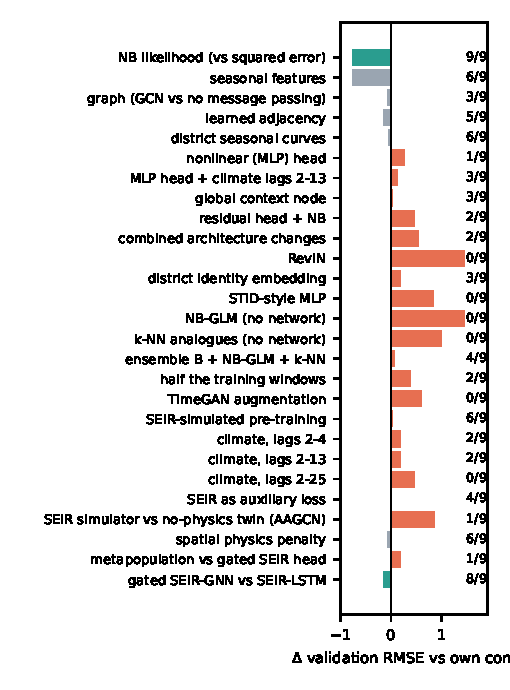
\includegraphics[width=\linewidth]{figures/fig_levers}
  \caption{Every lever's validation difference against its own control
  (Table~\ref{tab:levers}); win counts on the right. Green: negative and
  $\ge$7/9 wins. Grey: negative but inconsistent. Red: worse.}
  \label{fig:levers}
\end{figure}

\subsection{Hyperparameter tuning}
\label{sec:tuning}
In the main study every encoder and head uses the same fixed settings
(\S\ref{sec:impl}), chosen before the runs, so no model gets more tuning than another.
Before the prospective test we tuned each learned arm on the same grid and budget:
learning rate $\{10^{-3},3\times10^{-3}\}\times$ hidden size $\{32,64\}$, 108 runs per
arm on the nine development origins, selected on validation only. All three arms select
learning rate $3\times10^{-3}$ and $d=64$, the settings of the main study
(Table~\ref{tab:tuning}). The whole grid moves validation RMSE by at most 0.57, and the
ridge penalty of AR(3) by 0.12, so the conclusions do not hinge on tuning. Halving the
training windows costs $B$ 0.39 and a quarter of them 0.25 (Table~\ref{tab:levers}):
the models are not short of data.

\subsection{Computational analysis}
\label{sec:compute}
Table~\ref{tab:compute} gives the cost of each encoder and head. \model{} adds one
parameter and no measurable time per epoch (AAGCN 0.19 to 0.20 s). The SEIR branch adds
five parameters but roughly doubles the time per epoch on the light encoders (AAGCN
0.19 to 0.41 s), because it steps the simulator daily within every forecast week. The
encoders span three orders of magnitude, from AAGCN (2{,}873 parameters, 19 s per run)
to DCRNN (827{,}843 parameters, 3.6--4.1 s per epoch), and the smallest is the most
accurate. Every model trains on a free CPU; the full 810-run study takes 3.0 hours.

\subsection{Prospective evaluation, 2024--2026}
\label{sec:prospective}
The real test is weeks no setting was chosen on. We froze six arms and their settings
on development data, then parsed the new weeks (\S\ref{sec:newweeks}) and scored each
arm once on 85 forecast starts. The neural arms share one encoder, a Graph
WaveNet-style network with a learned adjacency~\cite{wu2019graphwavenet}, the
development finalist: \model{}, \model{} with the SEIR branch (the pre-registered
proposed model), and the residual head. Persistence, seasonal naive and an AR(3)
ridge regression complete the list.

Table~\ref{tab:prospective} gives the result. \textbf{No learned model beats
persistence on RMSE}: persistence scores 34.75, \model{} 35.43 and \model{}+SEIR 35.40,
differences that are not significant (\model{}+SEIR $+0.65$, $p_{\text{Holm}}=0.62$).
\textbf{The SEIR branch adds nothing} over \model{} ($-0.03$ [$-0.41$, $+0.12$],
$p_{\text{Holm}}=0.67$). On the secondary metrics the learned arms do better than
persistence (MAE 11.35 against 11.78, SMAPE 45.7 against 50.3), and every arm beats the
seasonal naive forecast by 26--28 RMSE. RMSE is dominated by the 2026 outbreak:
persistence scores 14.72, 20.05 and 160.51 in 2024, 2025 and 2026, and \model{} 14.32,
21.43 and 162.75. \model{} is better in the quiet year and worse in the outbreak, where
the next large move is not in the inputs. The development advantage of the SEIR arm over
persistence (27.34 against 28.54) does not carry over to later data.

Because the SEIR branch ties its no-SEIR twin, we present the simpler \model{} as the
framework. That choice is made after seeing the prospective result, and we state it as
such: the pre-registered finalist was the SEIR variant, and the two are equivalent.

\subsection{SEIR-GNN against SEIR-LSTM, and physics as structure}
\label{sec:seirgnn}
Behind the same gated SEIR head the graph beats the LSTM on three origins on
validation (ASTGCN $-0.54$, 9/9; AAGCN $-0.14$, 8/9), but on nine disjoint origins the
advantage is not robust to the encoder or the metric (Table~\ref{tab:nine}): ASTGCN's
holds on validation ($-0.62$, 8/9, $p=0.012$) and vanishes on test, and AAGCN's reverses.
Two further physics structures do not help: a spatial penalty on relative incidence
across borders ($-0.06$, 6/9) and a metapopulation SEIR head that couples districts
inside the dynamics ($+0.20$ against the gated SEIR head, 1/9, $\padj=0.020$). The data
explain why: on the district graph, Moran's $I$ is 0.29 for log cases but $-0.03$ for
weekly log growth, so levels cluster in space while changes in transmission do not.
% EXP-062: the nine-origin rows of tab:nine change after the week-index fix.

\subsection{The ceiling is informational}
\label{sec:ceiling}
The working encoders, the SEIR-LSTM and $k$-NN, which has no network and no training,
leave residuals that correlate 0.91--0.97 with $B$'s: the models make the same errors.
The remaining error is a lag on moves. $B$ under-predicts rising weeks by 11.5 cases and
over-predicts falling weeks by 10.1, and the top 5\% of district-weeks carry 54--67\% of
every model's squared error. That is what a mean-seeking objective produces on a
near-random-walk target whose next move is not in the inputs.

\subsection{Validation and test disagree, systematically}
\label{sec:valtest}
Across the eight families of runs, the configuration validation selects is worse than
persistence on test in five, and the best configuration on test is anchored to the
last observation in six (\model{}, residual, gated SEIR or $k$-NN). A 30-week validation
span immediately before each origin appears to reward fitting that span's level, which
does not carry into the next period. This is one reason we report the prospective test
as the decisive evidence.

%=============================================================================
% DISCUSSION AND CONCLUSION
%=============================================================================
\section{Discussion}
\label{sec:discussion}

\textbf{Why \model{} works, and what it cannot do.} Weekly dengue counts are close to a
random walk, so the most informative feature is the last value. A direct head must
carry that value through the encoder; STGAT, A3TGCN and DCRNN lose it and underfit.
\model{} hands the level to the output, so the encoder learns only the departure, and
the gate keeps a weak departure from pulling the forecast away from persistence. This is
why the same head repairs three different architectures, attention, recurrent and
diffusion based, by 6--16 RMSE. It also explains its limit: the anchor removes failure,
but it cannot create information. When the next large move is not in the inputs, as in
the 2026 outbreak, every model, \model{} included, lags it, and on RMSE no learned model
beats persistence on later data.

\textbf{Where physics helps a graph network, and where it does not.} On this target the
SEIR model cannot be the forecaster: a pure SEIR decoder inherits the poor
predictability of its force of infection, and 14--16\% of targets are out of its reach.
Inside the gated head it looked useful, because it made every encoder usable, but the
ablation shows that the anchor and gate do that work, and on later data the simulator
ties its no-physics twin. Coupling districts inside the dynamics does not help either,
because transmission changes have almost no local spatial structure at district-week
resolution. The graph itself adds 0.06 RMSE. The prior that matters is the one the data
already state: next week looks like this week.

\textbf{What the evaluation taught us.} Each of the following would have produced a
publishable positive result had it gone unchecked: the benchmark array leaks future data
through its row order and its climate channels; our own first SEIR-GNN pipeline compared
one origin against a three-origin baseline; the gated SEIR head's repair looked like
physics and was the anchor; the validation-selected model $B$ is worse than persistence
on test; and the SEIR arm's development advantage over persistence disappears on
2024--2026 data. We therefore recommend that dengue forecasting papers report
persistence, a matched no-physics control and, where possible, a prospective test.

\textbf{Limitations.} One country and one disease at district-week resolution. Three
origins cannot support claims at the origin unit, and the nine-origin test spans were
examined in earlier experiments, so they are not fresh. The prospective test is amended
(\S\ref{sec:newweeks}) and uses one encoder family; it is a single 2.4-year period
dominated by one outbreak year. The graph is the benchmark's hand-built adjacency, and
mobility data might couple districts differently. The SEIR branch uses fixed stage
durations and one initial susceptible fraction for every district.

\section{Conclusion}
We proposed \model{}, a persistence-anchored gated head for spatio-temporal dengue
forecasting that plugs into any encoder at the cost of one parameter, together with a
corrected, leakage-free dataset extended to 2026 with newly parsed reports. \model{} turns
three published ST-GNNs that are worse than persistence into usable forecasters, and
with a strong encoder it beats persistence on every paired run in the development
study. An ablation shows that the gain comes from the anchor and the gate; an SEIR
simulator in the same head adds nothing, on development data or on later weeks. On
weeks from 2024 to 2026 no learned model beats persistence on RMSE, though \model{} is
better on MAE and SMAPE. For district-level dengue in Sri Lanka, the useful prior is
persistence, not transmission dynamics, and the next gains must come from inputs that
anticipate outbreaks rather than from the architecture. The dataset, the notebook that
produces every development number, the pre-registrations and the experiment log are
available at \codeurl.


\balance
\bibliographystyle{ACM-Reference-Format}
\bibliography{refs}

\end{document}
